\documentclass{beamer}

\input{../../spec_files/course_preamble.tex}
\subtitle{Foundations of Neuro-Symbolic AI}
\date{Summer Term 2026}
\author[FONS]{Alex Goessmann}
\institute[]{
    University of Applied Science Würzburg-Schweinfurt (THWS)
%    Weierstrass Institute for Applied Analysis and Stochastic
}

\newcommand{\setslidetitledate}[2]{
    \title[#1]{
        \coursechapterone \\
        {\huge #1}
    }
    \date{#2}
}

\newcommand{\stantikzpic}[1]{
    \begin{center}
    \begin{tikzpicture}[scale=0.35, thick]
    #1
    \end{tikzpicture}
    \end{center}
}

%\newcommand{\techwstitle}{
%\small
%%Workshop \\
%Logik für Erklärbare KI:
%Technische Einführung in das ENEXA Projekt}
%\newcommand{\smalltechwstitle}{ENEXA Workshop}

%\newcommand{\techwsdate}{15.+16. July, 2024}

%\newcommand{\techwsauthors}{
%Alex Goessmann
%}

%\newcommand{\techwsinclude}{
%	\usepackage{../../spec/beamercolorthemeclaw}
%	\usepackage{/Users/alexgoessmann/Documents/ENEXA/latex_macros/beamer_template/beamerfontthemeclaw}
%	\usepackage{/Users/alexgoessmann/Documents/ENEXA/latex_macros/beamer_template/beamerinnerthemeclaw}
%	\usepackage{/Users/alexgoessmann/Documents/ENEXA/latex_macros/beamer_template/beamerouterthemeclaw}
%
%	\input{/Users/alexgoessmann/Documents/ENEXA/latex_macros/packages.tex}
%	\input{/Users/alexgoessmann/Documents/ENEXA/latex_macros/macros.tex}
%	\input{/Users/alexgoessmann/Documents/ENEXA/latex_macros/macros_tc.tex}
%	\input{/Users/alexgoessmann/Documents/ENEXA/latex_macros/tikz_blocks.tex}
%
%	\subtitle{\techwstitle}
%	\date[\techwsdate]{\techwsdate}
%	\author[\smalltechwstitle]{\techwsauthors}
%	\institute[]{\eupic}
%}

\newcommand{\coursechapterone}{I-Logical Approaches}
\newcommand{\coursechaptertwo}{II-Probabilistic Approaches}
\newcommand{\coursecahterthree}{III-Statistical Models of Knowledge Graphs}
\newcommand{\coursechapterfour}{IV-Quantum Machine Learning}

\newcommand{\techwschapterone}{I-Tensors}
\newcommand{\techwschaptertwo}{II-Probabilities}
\newcommand{\techwschapterthree}{III-Logics}
\newcommand{\coursechapterthree}{IV-Applications}

\newcommand{\eupic}{
    \begin{center}
    %
\includegraphics[width=4cm]{/Users/alexgoessmann/Documents/ENEXA/latex_macros/images/fundedEU.png}
    \end{center}
}

%\newcommand{\enexadateveublock}{
%    \begin{center}\begin{tikzpicture}
%    %\node [anchor=center] at (0,0) {\includegraphics[width = 1.5cm]{/Users/alexgoessmann/Documents/ENEXA/latex_macros/images/DATEV.png}};
%    %\node [anchor=center] at (2.5,0.5) {
\includegraphics[width = 3.5cm]{/Users/alexgoessmann/Documents/ENEXA/latex_macros/images/enexa.png}};
%    %\node [anchor=center] at (2.55,-0.5) {
\includegraphics[width = 3cm]{/Users/alexgoessmann/Documents/ENEXA/latex_macros/images/fundedEU.png}};
%    \end{tikzpicture}\end{center}
%}


%% OLD
\newcommand{\aselectionvariable}{L}
\newcommand{\vselectionvariable}{L}
\newcommand{\fselectionvariable}{L}
\newcommand{\cselectionvariable}{L}
\newcommand{\individualorder}{n}
\newcommand{\variableof}[1]{\indvariableof{#1}}
\newcommand{\sindex}{s}
\newcommand{\pindex}{p}
\newcommand{\oindex}{o}
\newcommand{\exquery}{q}
%\newcommand{\datapointof}[1]{x^{#1}}
\newcommand{\atomicqueryof}[1]{g_{#1}}
\newcommand{\facsystem}{\shortcatvariables}
\newcommand{\margprobof}[1]{\probat{#1}}
\newcommand{\mlnprobabilityof}[1]{\expdistof{#1}}
%\newcommand{\oldenexadateveublock}{
%	\begin{center}
%	\begin{minipage}{0.2\textwidth}
%		\begin{center}
%			\includegraphics[width = 2.5cm]{images/DATEV.png}
%		\end{center}
%	\end{minipage}
%	\begin{minipage}{0.55\textwidth}
%		\begin{center}
%			
\includegraphics[width=5.5cm]{images/enexa.png} \\
%			
\includegraphics[width=5.5cm]{images/fundedEU.png} \\
%		\end{center}
%	\end{minipage}
%	\end{center}
%}

\newcommand{\showoutlineatsection}{
    \AtBeginSection[ ]
    {
        \begin{frame}{Outline}
        \tableofcontents[currentsection]
        \end{frame}
    }
    %\begin{frame}{Outline}
    %\tableofcontents
    %\end{frame}

    \addtocounter{framenumber}{-1}
}

\tikzset{
    midarrow/.style={
        postaction={decorate},
        decoration={
            markings,
            mark=at position 0.5 with {\arrow{Straight Barb[length=4pt, width=5pt]}}
            % Or use {Stealth}, {To}, or {Latex[open]}
        }
    },
    midbackarrow/.style={
        postaction={decorate},
        decoration={
            markings,
            mark=at position 0.5 with {\arrow{<[Straight Barb[length=4pt, width=5pt]]}}
        }
    },
    >>-/.style={midarrow},
    <<-/.style={midbackarrow}
}

\newcommand{\drawtnreasonarchitecture}{
    \draw[dashed] (-30,15) -- (12,15) -- (12,-3) -- (-30,-3) -- (-30,15);

    \draw[] (-10,10) rectangle (10,14);
    \node [anchor=center] at (0,12) {\corelabelsize \spapplication{}};

    \node [anchor=west] at (-29,12) {\layerthreespec};
    \draw[dashed] (-30,9) -- (12,9);
    \node [anchor=west] at (-29,6) {\layertwospec};

    \draw[->] (6,10) -- (6,8);
    \draw[] (2,4) rectangle (10,8);
    \node [anchor=center] at (6,6) {\spreasoning{}};
    \draw[->] (6,4) -- (6,2);

    \draw[->] (-5,10) -- (-5,8);
    \draw[] (-10,4) rectangle (0,8);
    \node [anchor=center] at (-5,6) {\sprepresentation{}};
    \draw[->] (-5,4) -- (-5,2);

    \draw[dashed] (-30,3) -- (12,3);
    \node [anchor=west] at (-29,0) {\layeronespec};

    \draw[] (-10,-2) rectangle (10,2);
    \node [anchor=center] at (0,0) {\spengine};
}

\setchatwotitledate{
    Course Summary
}{
    July 6, 2026
}
\begin{document}

    {\frame[plain]{\titlepage}}
    \showoutlineatsection


    \section{AI in the tensor formalism}

    \begin{frame}{Definition of tensors}

        \begin{definition}[Tensor]
            A tensor of order $\catorder\in\nn$ with leg dimensions $\catdimof{\catenumerator}\in\nn$ (where $\catenumeratorin$) is a map
            \begin{align*}
                \hypercorewith \defcols \facstates \rightarrow \rr \, .
            \end{align*}
            The coordinate at the index tuple $\shortcatindices$ is the value $\hypercoreat{\indexedshortcatvariables}$.
        \end{definition}

        \begin{itemize}
            \item The order of the tensor is the number $\catorder$
            \item The number of coordinates is $\prod_{\catenumeratorin}\catdimof{\catenumerator}$
        \end{itemize}


    \end{frame}

    \begin{frame}{Visualization}

        {\bf Coordinatewise visualization:}
                    \begin{center}
                        \begin{tikzpicture}[scale=2]

                    \drawtextnode{-1.75}{0}{$\kbat{\catvariableof{0},\catvariableof{1},\catvariableof{2}}\,\,=$}

                    \node (A) at (0,0) [scale=1.5] {
                        $\begin{pmatrix}
                             0   &   1\\
                             1 & 0
                        \end{pmatrix}$
                    };
                    \node (A) at (1.25,0.3) [scale=1.5] {
                        $\begin{pmatrix}
                             0 & 0 \\
                             1 & 0
                        \end{pmatrix}$
                    };
                    \drawtextnode{2.25}{0}{$[\catvariableof{0},\catvariableof{1},\catvariableof{2}]$}
                    \draw[->,dashed] (-0.25,0.5) node[below] {\tiny $0$} -- (0.25,0.5) node [midway, above] {\tiny $X_1$} node[below] {\tiny $1$};
                    \draw[<-,dashed] (-0.6,-0.2) node[right] {\tiny $1$} -- (-0.6,0.2) node [midway, left] {\tiny $X_0$} node[right] {\tiny $0$};
                    \draw[->,dashed] (0,-0.5) node[above] {\tiny $0$} -- (1.25,-0.2) node [midway, below] {\tiny $X_2$} node[above] {\tiny $1$};
                        \end{tikzpicture}
                    \end{center}


                        {\bf Digrammatic visualization:}

                    \stantikzpic{
                        \drawtensorblock{0}{0}{3}{$\kb$}
                        \drawvwire{-2}{-1}{$\catvariableof{0}$}
                        \drawvwire{0}{-1}{$\catvariableof{1}$}
                        \drawvwire{2}{-1}{$\catvariableof{2}$}

                    }
    \end{frame}

    \begin{frame}{Tensor networks}

        We used the diagrammatic visualization to depict tensor networks on a hypergraph $\graph=(\nodes,\edges)$
        \begin{itemize}
            \item A set of nodes $\node$, decorated by variables $\catvariableof{\node}$
            \item A set of hyperedges $\edge\subset\nodes$ decorated by tensors $\hypercoreofat{\edge}{\catvariableof{\edge}}$
        \end{itemize}
        The toy accounting example was visualized by a hypergraph and a decoration by tensors as:
        \stantikzpic{
            \drawvariablenode{0}{0}{$\catvariableof{A2}$}{XA2}
            \drawvariablenode{5}{0}{$\catvariableof{A1}$}{XA1}
            \drawvariablenode{10}{0}{$\catvariableof{F}$}{XF}
            \draw (XF) to[bend right=40, edge node={node[midway,above] {$\edgeof{1}$}}] (XA1);
            \draw (XA1) to[bend right=40, edge node={node[midway,above] {$\edgeof{0}$}}] (XA2);
            \begin{scope}[shift={(0,-5)}]
                \drawtensorblock{2.5}{0}{2}{$\formulaof{0}$}
                \drawvwire{1}{-1}{$\catvariableof{A2}$}

                \drawtensorblock{7.5}{0}{2}{$\formulaof{1}$}

                \drawvwire{9}{-1}{$\catvariableof{AF}$}
                \draw(5,-2.5) to[bend right=-30] (4,-1);
                \draw(5,-2.5) to[bend right=30] (6,-1);
                \drawvariabledot{5}{-2.5}
                \drawvwire{5}{-2.5}{$\catvariableof{A1}$}
            \end{scope}
        }


    \end{frame}

    \begin{frame}{Definition of contractions}
        \begin{definition}[Contraction]
            Let $\tnetof{\graph}$ be a tensor network on a hypergraph $\graph=(\nodes,\edges)$.
            For any subset $\secnodes\subset\nodes$ we define the contraction to be the tensor
            \begin{align*}
                \contractionof{\tnetof{\graph}}{\catvariableof{\secnodes}}
            \end{align*}
            defined coordinatewise by the sum
            \begin{align*}
                \contractionof{\tnetof{\graph}}{\indexedcatvariableof{\secnodes}} =
                \sum_{\catindexof{\nodes\backslash\secnodes}\in\bigtimes_{\node\in\nodes\backslash\secnodes}[\catdimof{\node}]}
                \prod_{\edge\in\edges}\hypercoreofat{\edge}{\indexedcatvariableof{\edge}} \, .
            \end{align*}
        \end{definition}
    \end{frame}


    \begin{frame}{Tensor networks as a unifying language}

        {\bf Sparsity principle:} \emph{Tensor network decompositions}
        \begin{itemize}
            \item Logics: Syntactical description
            \item Neural: Circuit decompositions
            \item Probability: Representaion of independencies
        \end{itemize}

            {\bf Inference principle:} \emph{Tensor network contractions}
        \begin{itemize}
            \item Logics: Entailment
            \item Neural: Function evaluation
            \item Probability: Marginal and conditional distributions
        \end{itemize}

    \end{frame}


    \section{Neuro-Symbolic AI}

    \begin{frame}{Symbolic AI}

        \begin{block}{The symbolic paradigm}
            Humans reason in abstractions: Symbols
%            \begin{itemize}
%                \item Statements in languages
%                \item Logical
%            \end{itemize}
        \end{block}

        Advantages:
        \begin{itemize}
            \item Human interaction with models
            \item Guaranteed model behaviour
        \end{itemize}

        Challenges:
        \begin{itemize}
            \item Efficient model training
            \item Intractability of inference
        \end{itemize}

    \end{frame}

    \begin{frame}{Neural AI}

        \begin{block}{The neural paradigm}
            Interesting functions decompose into networks of easy functions.
        \end{block}


            {\bf Basis encodings}
        \begin{itemize}
            \item Represent arbitrary functions $\exfunction:\bigtimes_{\catenumeratorin}[\catdimof{\catenumerator}]\rightarrow\headstates$ as tensors:
            \begin{align*}
                \bencodingofat{\exfunction}{\headvariables,\shortcatvariables}
                = \sum_{\shortcatindicesin} \onehotmapofat{\exfunction(\shortcatindices)}{\headvariables} \otimes \onehotmapofat{\shortcatindices}{\shortcatvariables}
            \end{align*}
            \item Decomposition into circuits (see lecture I.6) is reflected in tensor network decompositions
        \end{itemize}
            {\bf Basis calculus}
        \begin{itemize}
            \item Contractions with one-hot encodings infer the functions
            \item Local contractions along the direction of the circuit suffice
        \end{itemize}
    \end{frame}


    \begin{frame}{Come to our workshop!}
        My group in Berlin will organize a workshop in Berlin (September 14-17, 2026) on {\bf Neuro-symbolic AI, Mathematical Reasoning and Agents}:
        \begin{center}
            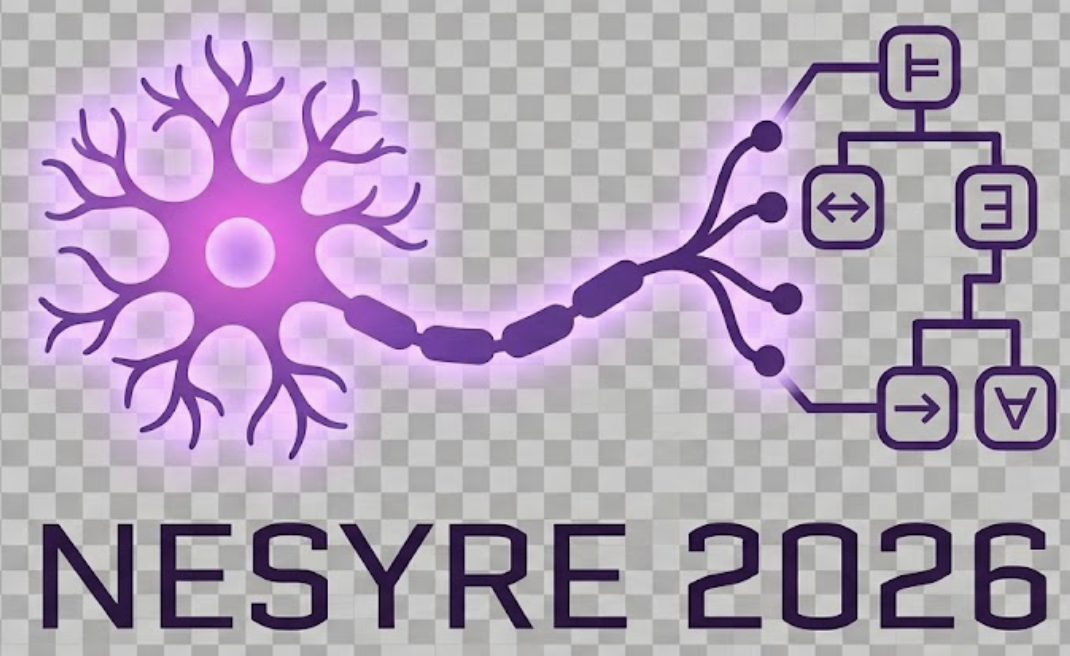
\includegraphics[width=5cm]{img/workshop-logo}
            \href{https://www.wias-berlin.de/workshops/NESYRE2026/}{https://www.wias-berlin.de/workshops/NESYRE2026/}
        \end{center}

        \hfill
        \begin{center}
            {\bf Please contact me if you would like to participate!} \\ (alex.goessmann@wias-berlin.de)
        \end{center}

    \end{frame}


    \section{Logical Approaches}

    \begin{frame}{Syntactical decompositions}


        \begin{block}{Sparsity by syntax}
            Syntactical representations of formulas provide means to decompose the tensor.
            The interesting formulas have syntactical representations of small size.
        \end{block}

        {\bf Example:} The basis encoding of the formula
        \begin{align*}
            \formulaat{\catvariableof{B},\catvariableof{E},\catvariableof{J},\catvariableof{M}}
            =(\catvariableof{B}\lor\catvariableof{E})\Rightarrow (\catvariableof{J}\lor\catvariableof{M})
        \end{align*}
        is decomposed as
        \stantikzpic{

            \draw[->-] (-1.5,-1)--(-1.5,1) node[midway,left] {\colorlabelsize $\catvariableof{B}$};
            \draw[->-] (0.5,-1)--(0.5,1) node[midway,right] {\colorlabelsize $\catvariableof{E}$};
            \draw[->-] (2.5,-1)--(2.5,1) node[midway,right] {\colorlabelsize $\catvariableof{J}$};
            \draw[->-] (4.5,-1)--(4.5,1) node[midway,right] {\colorlabelsize $\catvariableof{M}$};
            \draw (-2,1) rectangle (5, 3);
            \node[anchor=center] (text) at (1.5,2) {\corelabelsize $\bencodingof{\exformula}$};
            \draw[->-] (1.5,3)--(1.5,5) node[midway,right] {\colorlabelsize ${\headvariableof{\exformula}}$};

            \node[anchor=center] (text) at (7,2) {${=}$};


            \begin{scope}[shift={(11,0)}]

                \draw[->-] (-1,-1)--(-1,1) node[midway,left] {\colorlabelsize $\catvariableof{B}$};
                \draw[->-] (2,-1)--(2,1) node[midway,right] {\colorlabelsize $\catvariableof{E}$};
                \draw[->-] (6,-1)--(6,1) node[midway,right] {\colorlabelsize $\catvariableof{J}$};
                \draw[->-] (9,-1)--(9,1) node[midway,right] {\colorlabelsize $\catvariableof{M}$};

                \draw (-2,1) rectangle (3, 3);
                \node[anchor=center] (text) at (0.5,2) {\corelabelsize $\bencodingof{\lor}$};

                \draw[->-] (2,3) --(2,5) node[midway,right]{\colorlabelsize ${\headvariableof{B\lor E}}$};

                \draw (5,1) rectangle (10, 3);
                \node[anchor=center] (text) at (7.5,2) {\corelabelsize $\bencodingof{\lor}$};

                \draw[->-] (6,3) --(6,5) node[midway,right]{\colorlabelsize $\headvariableof{J \lor M}$};

                \draw (0.5,5) rectangle (7.5,7);
                \node[anchor=center] (text) at (4,6) {\corelabelsize $\bencodingof{\Rightarrow}$};

                \draw[->-] (4,7) -- (4,9) node[midway,right] {\colorlabelsize $\headvariableof{\exformula}$};
            \end{scope}

        }
    \end{frame}


    \begin{frame}{Logical Inference: Entailment}

        \begin{definition}[Entailment]
            Let $\kbat{\shortcatvariables}$ and $\formulawith$ be two propositional formulas.
            If for all worlds $\shortcatindices$, for which $\kbat{\indexedshortcatvariables}=1$, we also have $\formulaat{\indexedshortcatvariables}=1$, then we say that $\formula$ is entailed by $\kb$ and denote
            \begin{align*}
                \kb \models \formula \, .
            \end{align*}
        \end{definition}

            {\bf Contraction Criterion:}
        We have that a formula $\kbwith$ entails another formula $\formulawith$, if
        \begin{align*}
            \contraction{\kbwith,\lnot\formulawith} = 0 \, .
        \end{align*}

    \end{frame}


    \section{Probabilistic Approaches}

    \begin{frame}{Independence}

        \begin{definition}[Conditional Independence]
	        Given a joint distribution of variables $\catvariableof{\nodesa}$, $\catvariableof{\nodesb}$ and $\catvariableof{\nodesc}$, we say that $\catvariableof{\nodesa}$ and $\catvariableof{\nodesb}$ are independent given $\catvariableof{\nodesc}$ if for any index tuple $(\catindexof{\nodesa},\catindexof{\nodesb},\catindexof{\nodesc})$
            \begin{align*}
                \condprobof{\indexedcatvariableof{\nodesa},\indexedcatvariableof{\nodesb}}{\indexedcatvariableof{\nodesc}}
                =  \, & \condprobof{\indexedcatvariableof{\nodesa}}{\indexedcatvariableof{\nodesc}}\\
                & \cdot \condprobof{\indexedcatvariableof{\nodesb}}{\indexedcatvariableof{\nodesc}}   \, ,
            \end{align*}
            We denote this situation by
            \begin{align*}
                \condindependent{\catvariableof{\nodesa}}{\catvariableof{\nodesb}}{\catvariableof{\nodesc}} \, .
            \end{align*}
        \end{definition}

            {\bf Contraction criterion:} We have $ \condindependent{\catvariableof{\nodesa}}{\catvariableof{\nodesb}}{\catvariableof{\nodesc}} $ if and only if
        \begin{align*}
            \condprobat{\catvariableof{\nodesa},\catvariableof{\nodesb}}{\catvariableof{\nodesc}}
            = \contractionof{
                \condprobat{\catvariableof{\nodesa}}{\catvariableof{\nodesc}},
                \condprobat{\catvariableof{\nodesb}}{\catvariableof{\nodesc}}
            }{\catvariableof{\nodesa},\catvariableof{\nodesb},\catvariableof{\nodesc}} \, .
        \end{align*}
    \end{frame}


    \begin{frame}{Graphical models: Visualizing independencies in hypergraphs}

        {\bf Bayesian networks (directed hypergraphs):}
        \begin{itemize}
            \item We choose any enumeration $[\catorder]$ of the nodes respecting the direction (outgoing nodes after incoming nodes)
            \item To each directed hyperedge we define the incoming nodes as parents to the outgoing node
            \item Any Bayesian network on the hypergraph satisfies for each $\catenumeratorin$ the conditional independencies
            \begin{align*}
                \condindependent{\catvariableof{\catenumerator}}{\catvariableof{[\catenumerator]\backslash\parentsof{\catenumerator}}}{\catvariableof{\parentsof{\catenumerator}}}
            \end{align*}
        \end{itemize}
            {\bf Markov networks (undirected hypergraphs):}
        \begin{itemize}
            \item Disjoint node sets $\nodesa$ and $\nodesb$ are separated by $\nodesc$, if any path from $\nodesa$ to $\nodesb$ passes a node in $\nodesc$.
            \item Any Markov network on the hypergraph satisfies for any node sets $\nodesa$ and $\nodesb$ separated by $\nodesc$
            \begin{align*}
                \condindependent{\catvariableof{\nodesa}}{\catvariableof{\nodesb}}{\catvariableof{\nodesc}}
            \end{align*}
        \end{itemize}
    \end{frame}

\end{document}